\documentclass[letter]{article}
\def\baselinestretch{1.5}
\usepackage{fullpage}
\usepackage{natbib}
\usepackage{graphicx}
\author{Benjamin R. Hillman}
\title{Improving subgrid-scale clouds and precipitation in large-scale models: thesis proposal}

\begin{document}
\maketitle
\section{Introduction}
% THESIS: ambiguities in radiative fluxes and in simulated satellite-observable cloud properties from large-scale models are reduced by improving the treatment of resolved cloud and precipitation structure and overlap.

Clouds are a key piece of the global climate system, but accurate modeling of clouds in large-scale models is difficult, and cloud feedbacks in global climate models (GCMs) are recognized as a primary contributor to inter-model differences in responses to climate forcings \citep[e.g.,][]{cess_et_al_1990,bony_and_dufresne_2005,williams_and_webb_2009,medeiros_et_al_2008}.

The complexity of simulating the climate system with current computational resources limits GCM resolutions to tens or hundreds of kilometers, but clouds occur and vary on much smaller spatial scales. This means that traditional GCMs are unable to resolve individual clouds, and instead descriptions of clouds in GCMs are limited to large-scale statistical summaries of cloud properties on the scale of the model grid \citep{randall_et_al_2003}. But radiative fluxes depend on cloud properties in a non-linear manner and so the details of the unresolved structure and variability of clouds is important for model radiative transfer parameterizations \citep[e.g.][]{barker_et_al_1999}. Most GCMs however, fail to completely account for unresolved cloud structure and variability in a sufficient manner.

% THESIS
The goal of this project is to reduce errors in radiative fluxes and simulated satellite-observable cloud diagnostics in large-scale models by improving the treatment of unresolved clouds and precipitation.

\section{Background}
The description of clouds in GCMs typically includes profiles of partial cloudiness (cloud area fraction by level) and the in-cloud liquid and ice cloud condensate \citep[e.g.][]{cam3_description,cam4_description}. The gridbox mean description of clouds does not in itself specify how the clouds should be distributed horizontally and vertically within model gridboxes, and characterization of the unresolved structure depends on additional assumptions about how clouds in overlapping layers are aligned vertically and how cloud properties vary within model gridboxes.

Early radiative transfer parameterizations in large-scale models used relatively simple assumptions about how subgrid-scale overlapping cloudy layers align vertically \citep[e.g.][]{collins_2001}. These include maximum overlap, in which the cloudy portions of overlapping cloudy layers are assumed to be perfectly correlated (i.e., vertically projected cloud area is minimized); random overlap, in which the cloudy portions of overlapping cloudy layers are uncorrelated; and the popularly used maximum-random overlap, in which adjacent cloudy layers are maximimally overlapped but layers separated by at least one clear layer are randomly overlapped \citep{geleyn_and_hollingsworth_1979}. The maximal-random overlap assumption in particular has been used in a number of GCMs \citep[e.g.][]{cam3_description,cam4_description,cam5_description}. However, these assumptions have been shown to be insufficient to capture the complexity of clouds seen in observations \citep[e.g.][]{hogan_and_illingworth_2000,mace_and_benson-troth_2002,barker_2008}, and sensitivity tests using high resolution model simuations have shown that unrealistic overlap assumptions can lead to large errors in calculated fluxes and heating rates \citep{barker_et_al_1999,wu_and_liang_2005}.

Subgrid-scale variability in cloud condensate is often completely neglected in GCMs, despite the fact that clouds can exhibit large variability on scales much smaller than GCM gridboxes \citep[e.g.][]{stephens_and_platt_1987}. This is problematic because radiative fluxes and heating rates calculated from model radiative transfer parameterizations are sensitive to subgrid-scale variations in cloud condensate \citep[e.g.][]{barker_et_al_1999,wu_and_liang_2005,oreopoulos_et_al_2012}. The sensitivity to both cloud overlap and condensate variability emphasizes the need to provide descriptions of clouds in large-scale models radiative calculations that include both horizontal variability in cloud properties and more realistic cloud overlap.

One way to account for subgrid-scale variations in cloud structure and condensate amount is to actually generate ensembles of subcolumns from the gridbox mean properties and calculate the radiative fluxes and heating rates on each generated subcolumn independently using the independent column approximation \citep[ICA;][]{cahalan_et_al_1994}. This can get incredibly computationally demanding when the number of columns gets even moderately large due the need to integrate over a large number of spectral intervals for each subcolumn, but \cite{pincus_et_al_2003} introduced an approach that reduces the computational burden substantially by stochastically sampling both cloud state and spectral interval simultaneously. This approach, known as the Monte Carlo Independent Column Approximation (McICA), allows for fast ICA-like radiative transfer calculations that can treat inhomogeneous clouds and has been incorporated into the widely used RRTMG radiation package and used in a number of state-of-the-art models \citep{iacono_et_al_2008,von_salzen_et_al_2012,cam4_description,cam5_description,donner_et_al_2011,navgem_description},

McICA separates the treatment of cloud structure and variability from radiative transfer parameterization, leaving the task of describing complex cloud structure and variability up to subcolumn sampling schemes. In principle, arbitrarily complex cloud geometries and condensate distributions can be generated by incorporating more sophisticated subcolumn schemes. However, the subcolumn schemes currently used in most GCMs make many of the same simplifications used by earlier models, including maximum-random overlap and homogeneous cloud properties \citep[e.g.][]{cam4_description,cam5_description}. Improved subcolumn schemes are needed to take full advantage of the flexibility offered by McICA.

Unresolved cloud structure and condensate variability is important not only for calculations of radiative fluxes, but also for cloud diagnostics commonly used for evaluation of model cloud properties themselves. Satellite instrument simulators such as those provided by the CFMIP Observational Simulator Package \citep[COSP;][]{bodas-salcedo_et_al_2011} are often used to remove ambiguities in model evaluation studies that arise from uncertainties and limitations in satellite retrievals of cloud properties by producing psuedo-observations from the model state that are more directly comparable to the satellite observations \citep[e.g.][]{klein_and_jakob_1999,webb_et_al_2001,zhang_et_al_2005,zhang_et_al_2010,kay_et_al_2012,klein_et_al_2013}. A key first step in simulating satellite observations from GCM cloud properties is accounting for the mismatch in resolved scales between the satellite pixel and model resolution by downscaling the gridbox mean cloud properties. This is done in COSP by stochastically generating subcolumns consistent with an overlap assumption to account for correlations in overlapping cloudy layers in the same manner as described for McICA above. However, the current implementation of COSP allows for only the simple maximum, random, or maximum-random overlap, and treats subcolumn clouds and precipitation as homogeneous. To the extent that the simulated satellite-observables are sensitive to these assumptions, failing to accurately characterize the subgrid cloud structure and condensate variability potentially introduces ambiguities into satellite-model comparisons. This problem deserves a closer look to build confidence in conclusions derived from these evaluation efforts. A strategy for assessing these sensitivities and for improving the representation of subgrid scale cloud and precipitation overlap and variability is presented in the following sections.

\section{Proposed work}

\subsection{Sensitivity of simulated satellite-observable cloud diagnostics to unresolved clouds and precipitation}
A straightforward analysis method is used to evaluate the sensitivity of COSP diagnostics to assumptions about subgrid-scale cloud and precipitation overlap and variability. The subcolumn sampling scheme within the COSP code can be bypassed by providing fields with resolved clouds and precipitation. Assumptions about variability and overlap can then be mimicked by modifying the resolved fields used as input to the simulators, and the differences in the outputs can be taken to represent sensitivities to the modeled assumptions.

Previous studies have used cloud resolving model simulations in a similar manner to evaluate the sensitivity of radiative fluxes and heating rates to overlap and unresolved variability \citep[e.g.][]{barker_et_al_1999,wu_and_liang_2005}. A more comprehensive sampling of different cloud regimes is obtained for this study by using output from the Multi-scale Modeling Framework \citep[MMF;][]{khairoutdinov_and_randall_2001,randall_et_al_2003}. The MMF replaces the cloud parameterizations in a traditional GCM with a 2D cloud resolving model in each gridbox. This provides global fields with resolved subgrid structure that can be passed directly to the individual instrument simulators within COSP.

In order to separately evaluate the sensitivity to overlap and heterogeneity, the following sets of modified fields are performed:
\begin{itemize}
    \item CRM: The original CRM fields within each gridbox of the MMF are used as inputs to the individual instrument simulators in COSP.
    \item CRM-HOM: hydrometeor mixing ratios are replaced with in-cloud averages, but the locations of hydrometeors (both cloud and precipitation) are retained from the full CRM fields (i.e., occurrence overlap is retained from the CRM).
    \item CRM-RES: hydrometeor mixing ratios are re-sampled from the full CRM fields, but the locations of hydrometeors (both cloud and precipitation) are retained from the full CRM fields.
    \item MRO-HOM: hydrometeor mixing ratios and cloud optical properties are first averaged to produce gridbox means, similar to what a GCM would diagnose. Subcolumns are then regenerated consistent with the commonly used maximum-random overlap assumption, and homogeneous cloud properties (the gridbox means) are assigned to the cloudy subcolumns.
\end{itemize}
An example of these different fields obtained from a single grid cell from the MMF is shown in Figure \ref{subgrid_fields}. The only difference between the CRM and CRM-HOM fields is that the CRM-HOM fields have homogeneous cloud and precipitation properties, so differences in COSP diagnostics calculated from these two cases represent the sensitivity to unresolved variability in cloud and precipitation properties alone. Differences between the diagnostics calculated from the CRM-HOM and MRO-HOM fields represent errors arising due to assumptions about cloud (and precipitation) overlap. The CRM-RES modification destroys any correlation between condensate amount at different levels, so differences between the CRM and CRM-RES simulations represent errors arising due to condensate amount overlap and the overlap between hydrometeor condensate of different types (clouds and precipitation).

\begin{figure}
\centering
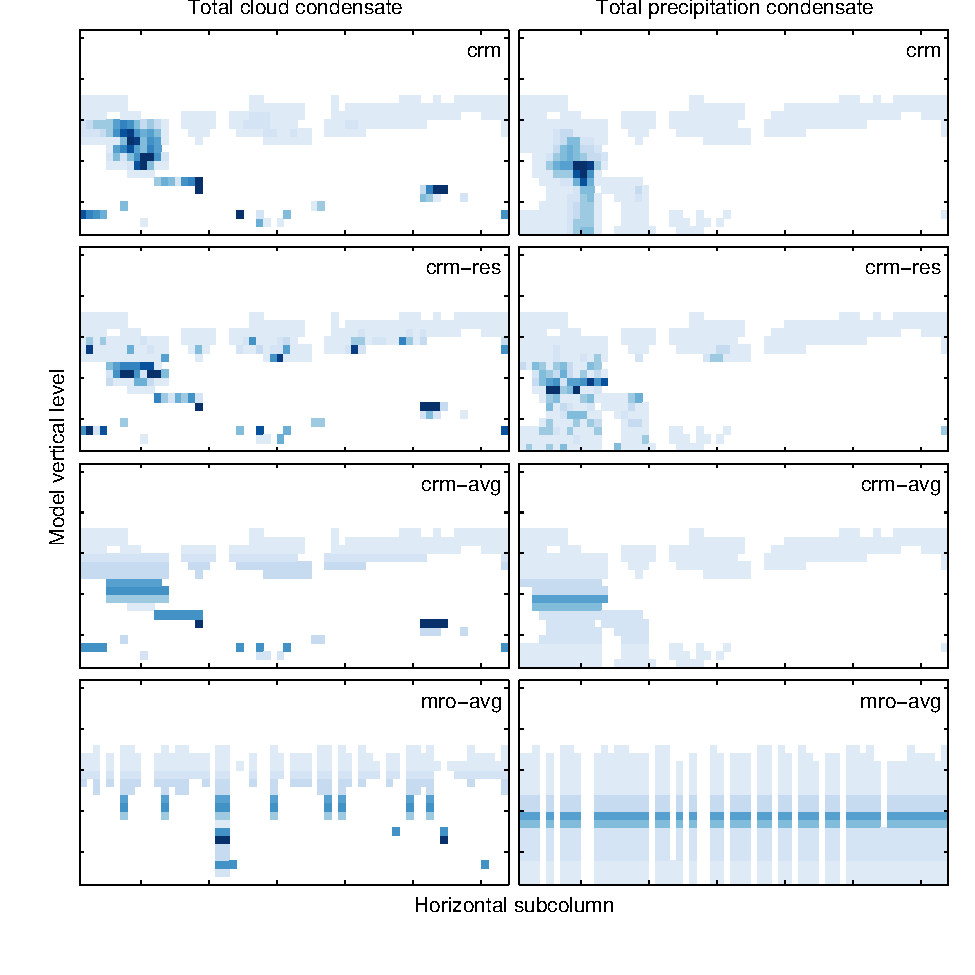
\includegraphics{test_subgrid.pdf}
\caption{Total cloud and precipitation condensate mixing ratios modified from the embedded CRM condensate mixing ratios within a single MMF gridbox.}
\label{subgrid_fields}
\end{figure}

Simulated CloudSat \citep{stephens_et_al_2002} radar reflectivity factor with height histograms from these four cases are shown in Figure \ref{cfadDbze94_figure}. The CRM-RES simulation too many hydrometeors relative to the outputs from the full CRM case in middle levels above about 7 km with radar reflectivity factor between $-20$ and $10$ dBZ. Because these cases have the same level-by-level PDF of condensate amount by construction, differences between these two cases arise due to differences in the alignment of condensate amount between levels. The differences shown here highlight the importance of accounting for this alignment in an improved subcolumn generator. 

The CRM-AVG simulation has too many hydrometeors along the entire characteristic curve of the histogram relative to the CRM case, but this is especially evident at low levels and for radar reflectivity factor greater than $0$ dBZ. Hydrometeros in this height and reflectivity range are attributed to low-level drizzle and rain \citep{marchand_et_al_2009}, and the overestimation of hydrometeor occurrence in this mode in the CRM-AVG simulation relative to the CRM case would imply that there is too much precipitation in the CRM-AVG case. However, these cases were drawn from the same CRM simulation and by construction the precipitation fraction at each level in each large-scale gridbox (number of subcolumns containing precipitation divided by total number of subcolumns) is consistent between the two cases. This emphasizes the need to account for subgrid variability in condensate amounts in order to be able to draw meaningful conclusions from simulator comparisons.

The MRO-AVG has even larger hydrometeor occurrence along the characteristic curve than the CRM-AVG simulation, especially for low-level hydrometeors with radar reflectivity greater than $0$ dBZ. This suggests that the MRO-AVG simulation has even more widespread precipitation than the already too high CRM-AVG simulation. This is likely true in the MRO-AVG simulation due to the simple treatment of precipitation subcolumn generation used here, in which precipitation is not constrained by the actual precipitation fraction, but assigned to any level in a column in which the precipitation fraction is non-zero and contains cloud in the current column or precipitation in the column above. This likely leads to an overestimation of precipitation occurrence (suggested by the single-column example shown in Figure \ref{subgrid_fields}), and this is consistent with the overestimation of hydrometeors with large radar reflectivity factor shown here. \cite{dimichele_et_al_2012} demonstrate considerable sensitivity of simulated radar reflectivity (using a different simulator) to different approaches of generating precipitation subcolumns. Yuying Zhang and Stephen Klein have been working on an improvement to this treatment of precipitation that constrains the generated subcolumn precipitation to a precipitation fraction diagnosed from the model. Results from their own sensitivity tests to their improvements are in preparation, and it will be interesting to see how these changes affect the sensitivity to subgrid-scale variability shown here. 

%, while simulated MISR, ISCCP, and MODIS cloud top height/pressure histograms are shown in Figure \ref{cth_hist}. These results suggest that the simulated radar reflectivity is sensitive to the subgrid variability in condensate, but less sensitive to the cloud occurrence overlap, while simulated MISR, ISCCP, and MODIS histograms of CTP and cloud amount are more sensitive to both subgrid condensate variability and cloud occurrence overlap. Differences in the simulated radar reflectivity between the MRO-AVG and CRM-AVG outputs are complicated by the strong sensitivity of the radar reflectivity to precipitation, which is treated in a very simple manner in the subcolumn generator used here. Precipitation is assigned to subcolumns at levels in which the precipitation fraction is non-zero and either contain cloud at the current level or precipitation at the level directly above. As shown in Figure \ref{subgrid_fields}, this can overestimate the precipitation fraction of the regenerated subcolumns. Nonetheless, this work, along with the sensitivity of radiative fluxes and heating rates identified by others, improvements to the treatment of subgrid-scale cloud and precipitation proposed in the following section.

\begin{figure}
\centering
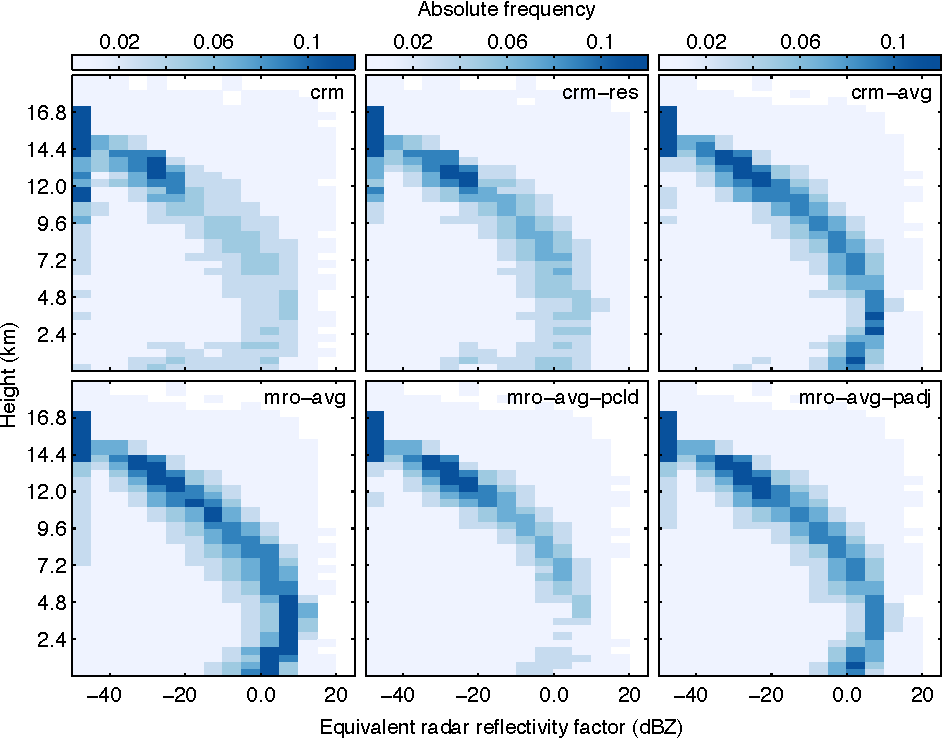
\includegraphics{radar_alt40-dbze.pdf}
\caption{Simulated CloudSat radar reflectivity factor with height histogram for the Tropical Warm Pool region.}
\label{cfadDbze94_figure}
\end{figure}

Figure \ref{all_cth} shows simulated ISCCP, MODIS, and MISR cloud top presure (or height, in the case of MISR) histograms for the same Tropical Warm Pool region from each of these cases. There are some noteworthy differences in the simulated cloud top height between the different cases, especially for the high-topped clouds. Cloud in the highest cloud top pressure bin is underestimated and the second highest cloud top pressure bin underestimated in both cases with averaged optical properties (CRM-AVG and MRO-AVG) relative to the cases without the averaging, with differences up to about $5\%$ cloud cover. The MODIS-simulated cloud top pressure has smaller differences that are not consistent with the ISCCP-simulated cloud top pressure. The largest differences are in the MISR-simulated cloud top height, and all of the modified cases overestimate clouds with top between $11$ and $13$ kilometers relative to the full CRM case. The MRO-AVG has the largest departure from the cRM case, and also underestimates mid-level and low-level clouds. Differences between the MRO-AVG and CRM-AVG simulations suggest that overlap does play a role in these differences, but the differences between the CRM and the CRM-AVG cases suggest that the subgrid variability in optical properties is important as well. Overall, the simulated ISCCP, MODIS, and MISR cloud top height diagnostics appear to be less sensitive to the subgrid variability and condensate overlap than the simulated radar reflectivity, but there are some differences that need to be explored further. It is unclear from this simple analysis whether these differences are significant or if they are greater in magnitude than the uncertainty in the observations or simulators themselves. A separate study is underway evaluate the sensitivity of the MISR simulator comparisons using hydrometeor profiles derived from a combination of CloudSat and CALIPSO data, which will help determine the limits to which we can assign biases to significant differences between models and observations.

%The MISR simulator includes an algorithm to mimic the tendency for MISR to see through thin, high-topped cloud and retrieve the cloud tops of lower-topped thicker clouds in the case of profiles with cloud in multiple levels of the atmosphere.
\begin{figure}
\centering
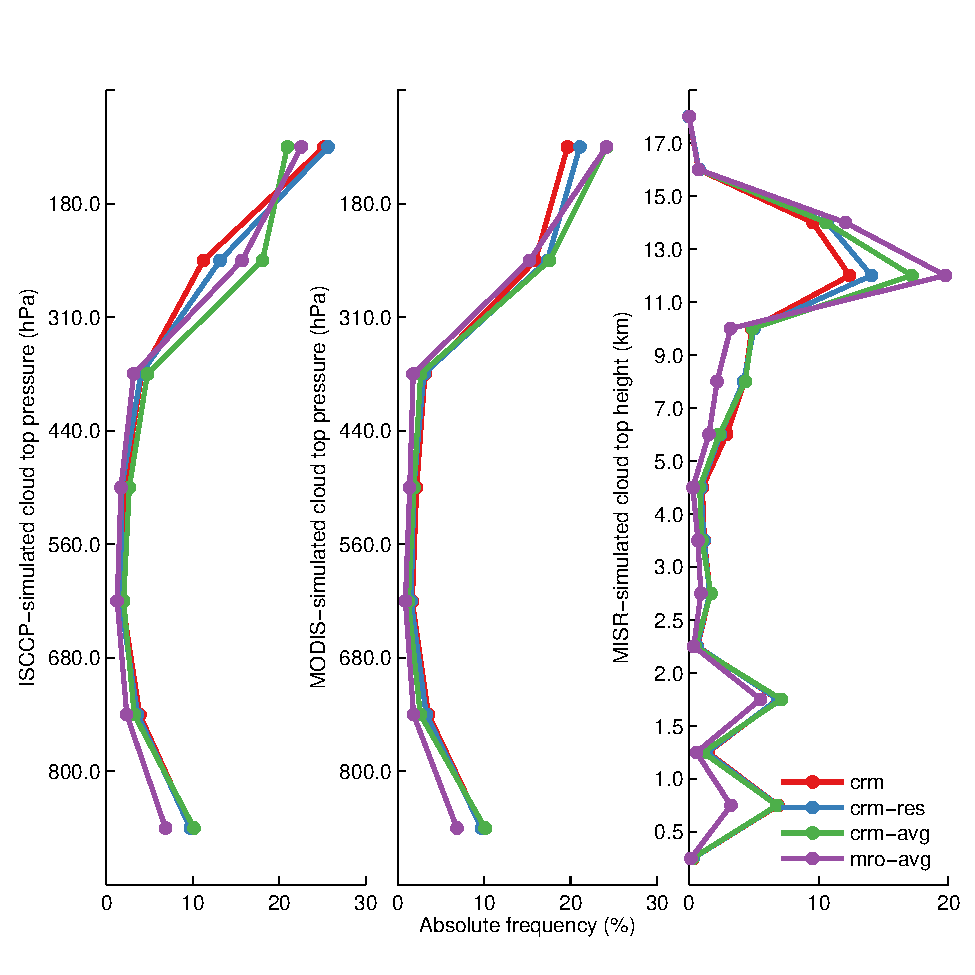
\includegraphics{all_cth.pdf}
\caption{Simulated ISCCP, MODIS, and MISR clout top pressure (height) histograms for the Tropical Warm Pool region.}
\label{all_cth}
\end{figure}

The sensitivities identifed in this section motivate improvements to the treatment of subgrid variability and overlap for use in COSP.

\subsection{Improving treatment of cloud and precipitation overlap and subgrid scale variability}
\cite{raisanen_et_al_2004} present the details of a scheme that can generate cloudy subcolumns with more flexible occurrence overlap and variable in-cloud condensate. Their scheme allows for overlap that is a combination of maximum and random \citep[e.g.][]{hogan_and_illingworth_2000}, which has been demonstrated to better fit both observations and high resoluation model simulations than simple maximum-random overlap \citep{hogan_and_illingworth_2000,mace_and_benson-troth_2002,pincus_et_al_2005,barker_2008}. The weighting between maximum and random overlap is determined by a decorrelation length scale that describes how overlap changes from maximum to random with separation distance. Variable in-cloud condensate for subcolums is possible if the probability distribution function (PDF) of condensate can be input to the subcolumn generator. The vertical alignment of condensate amount is determined by a separate decorrelation length scale that describes how the rank correlation of condensate amount between layers varies with separation distance. \cite{raisanen_et_al_2004} demonstrate improvements in radiative fluxes calculated using their improved subcolumn generator by resampling subcolumns from high-resolution model output with decorrelation depths and condensate distribution derived directly from the high-resolution model output.

\cite{oreopoulos_et_al_2012} test the sensitivity of a global climate model to improved subgrid clouds using the \cite{raisanen_et_al_2004} generator. They derive approximate decorrelation depths that vary with latitude and season from an analysis of CloudSat data \citep{stephens_et_al_2002}, and use beta distributions to describe the variability of in-cloud condensate. Their results suggest that improvements in radiative fluxes due to implementation of this scheme may be significant, but their simple latitude and seasonal dependence of decorrelation depths are not guaranteed to hold in a changing climate, and parameterization of these quantities in terms of model fields is probably a better approach for operational use in a model intended to aid understanding of the climate system in response to changes. \cite{pincus_et_al_2005} derive decorrelation depths from cloud resolving model data, and suggest parameterizing these in terms of large-scale fields such as wind shear and convective strength. They provide such a parameterization, but limited to a single domain over the ARM SGP site. Nonetheless, this is a good start, and this is an attractive avenue for further parameterization of these quantities. A major contribution of the present work will be to provide a more comprehensive characterization of the subgrid-scale structure of clouds and precipitation.

Another promising subgrid method is the Subgrid Importance Latin Hypercube Sampler \citep[SILHS;][]{larson_et_al_2005,larson_and_schanen_2013}, which can generate stochastic subcolumns from an assumed PDF of an arbitrary number of mixing ratios and has been set up to work with the Cloud Layers Unified By Binormals \citep[CLUBB;][]{golaz_et_al_2002} in the development version of CAM5 (Peter Caldwell, personal communication).

I propose a characterization of overlap statistics using output from the MMF to add to the work already done by others, and to separately diagnose overlap of clouds and precipitation which is difficult to do using radar observations as done by \cite{hogan_and_illingworth_2000},\cite{mace_and_benson-troth_2002}, and \cite{barker_2008}. The advantage of using the MMF for these studies is that it provides a complete description of subgrid-scale clouds and precipitation across all regimes and inludes the large-scale fields available in a traditional GCM, which will likely be useful for parameterizating the overlap characteristics. The limitation with this approach is that the MMF is still a model, and may not completely capture the complexity of the real atmosphere. In order to address this issue, I also plan to use hydrometeor occurrence profiles derived from CloudSat \citep{stephens_et_al_2002} and CALIPSO \citep{winker_et_al_2007} observations to independently derive overlap statistics in a similar manner as done by \cite{barker_2008} to compare with my characterization of overlap derived from MMF output. The goal is for this analysis to result in a parameterization of decorrelation lengths for both cloud and precipitation occurrence and condensate overlap based on large-scale fields. As suggested in the previous section, treating the precipitation in a more realistic manner will be important in accurately simulating radar reflectivities.

Subgrid-scale variability of cloud and precipitation condensate amount will also need to be characterized. With recent interest in PDF-based cloud parameterizations \citep[e.g.][]{tompkins_2002}, it makes sense to connect the subcolumns used by the radiative transfer and COSP modules to those used in the cloud physics parameterizations directly. There is an on-going project to implement the Cloud Layers Unified By Binormals \citep[CLUBB][]{golaz_et_al_2002} into the National Center for Atmospheric Research (NCAR) Community Atmosphere Model (CAM), which would naturally provide the subgrid-scale variability in total water and rain water mixing ratios needed. Work as already been done to pass PDFs of condensate from CLUBB to the radiation code in the development version of CAM5 (Andrew Gettelman, personal communication), and it would likely be straightforward to extend this to either pass the subcolumns generated by the McICA code to COSP, or to similarly pass the PDFs of condensate to an improved COSP subcolumn sampler to include the subgrid variability.

In the interest of also providing a stand-alone parameterization for use in offline calculations of simulator diagnostics using COSP, I also propose to develop an independent characterization of subgrid-scale cloud and precipitation variability. I plan to base this on output from both the MMF and available observations. The basic outline of this is to use the MMF to provide a first-guess at the distribution, and then to compare that to observations where possible. CloudSat reflecitivies have been used by others to derive variability parameters \citep{oreopoulos_et_al_2012}, but these carry large uncertainties due to the strong sensitivity to precipitation and difficulty in separating clouds from precipitation using radar reflectivity alone. Because of this, it might be necessary to look at variability derived from in-situ measurements as an additional check of variability derived from MMF output.

\subsection{Sensitivity of radiative fluxes and COSP simulator diagnostics to improvements in the treatment of cloud and precipitation overlap and subgrid-scale variability}
Following the characterization of overlap statistics and subgrid-scale variability, the next step is to implement the improved scheme into COSP and into a GCM and test the sensitivity of the fluxes and simulated satellite-observables to the improvements. 

Implementation of the improved subgrid treatment is relatively straightforward in the stand-alone COSP code, and the new subcolumn generator can just replace the ``SCOPS'' and ``PREC\_SCOPS'' modules in that code. For use in CAM5, however, these modules should be bypassed and common subcolumns between COSP and the McICA radiative transfer code should be used to enforce consistency between the radiative transfer and the (radiatively-important) satellite-observable cloud diagnostics. 

As mentioned above, the infrastructure to sample subcolumns with variable condensate from CLUBB PDFs has already been implemented in the development version of the CAM5. It should then be straightforward to either pass subcolumns with subgrid variability generated for the radiation code to COSP, or to pass CLUBB PDFs of condensate to COSP for generation of the subcolumns. This will allow for concurrent evaluation of the sensitivity of both radiative fluxes and COSP diagnostics to changes in the treatment of the subgrid cloud and precipitation structure and variability, with variability specified by the CLUBB physics parameterization. It is not clear yet whether or not their implementation generates subcolumns of precipitating hydrometeors. This will be important for the COSP diagnostics, and may need to be added or improved depending on what they have done.

Sensitivity of the COSP diagnostics will be tested alongside the radiative fluxes and heating rates in the context of the CAM5 implementation. The stand-alone COSP subcolumn scheme will be tested using MMF output and a similar framework as described above for the baseline sensitivity tests of the COSP outputs.

%Implementing generalized overlap and in-cloud variability in condensate using the \cite{raisanen_et_al_2004} method requires specification of the overlap parameter that determines the weighting between maximal and random overlap, the PDF of condensate distribution, and the rank correlation between condensate amounts in different layers. \cite{hogan_and_illingworth_2000} suggest that the overlap parameter $\alpha$ can be approximated as a decaying exponential function of separation distance $\Delta z$ between layers, such that determining $\alpha$ is akin to specify the e-folding depth $z_0$. \cite{raisanen_et_al_2004} suggest that the rank correlation $r$ can likewise be approximated as an exponential function of separation distance between layers, with a separate e-folding depth $z_{r}$.

%After performing a baseline assessment, the next and probably most difficult step is to develop or select a parameterization of subgrid-scale cloud variability. I think the most natural way to integrate a model for subgrid-scale variability into radiative schemes used in large-scale models is to take a PDF-based approach for use with the McICA. Such a method would presumably prescribe a PDF of cloud optical properties based on the large scale atmospheric state and the grid-box mean quantities. I believe such a scheme has already been implemented to an extent in the latest climate model produced by CCCma, the CanAM4 \citep{von_salzen_et_al_2012}, which assumes a gamma distribution for the cloud condensate based on previous studies such as that by \cite{barker_1996}. I have had some preliminary conversations with Jason Cole at CCCma about this, and he is interested in expanding upon their parameterization and further discussing possibilities with us for how to do this. I'm not completely clear on the details of the current implementation, and more discussions on this need to take place.

%The aforementioned strategy may provide for a flexible implementation applicable to a range of climate models, and in particular may lend itself to development of an improved stand-alone subcolumn generator for COSP, but with recent interest in PDF-based cloud parameterizations it may make more sense to connect the subcolumns used by the radiative code to those used in the cloud physics parameterizations more directly. There is an on-going project to implement the Cloud Layers Unified By Binormals \citep[CLUBB][]{golaz_et_al_2002} into CAM, which would naturally provide the subgrid-scale variability we are after \citep{wood_2012}. Rob Wood expressed interest in discussing this further and keeping in touch on this front.

%\subsection{Implementing in a large scale model}
%The next step would be to implement the parameterization of subgrid-scale clouds into a large-scale model and to test the impact of the changes on the calculated fluxes and heating rates and the simulated cloud diagnostics. Again, I think CAM5 would make an excellent test-bed for this, since much of the machinery is already in place (McICA, and on-going development to include a PDF-based cloud scheme).

%In the case of developing a new subcolumn generator that is somewhat independent of the cloud physics parameterization (i.e., the first method described in the previous subsection, not the integrated CLUBB method), the parameterization can be tested before being implemented into a particular large-scale model. This can be done by using fields generated by a cloud resolving model, and applying various averaging methods and radiative transfer solvers. One strategy would be to take a domain maybe the size of a typical climate model grid-box for a particular case. A benchmark calculation might be to run an ICA radiative transfer code on the fully resolved CRM fields. One test might consist of averaging the CRM fields over the horizontal domain, assigning subcolumns using the new subcolumn generator, and running the ICA code on the generated subcolumns and comparing the fluxes and heating rates with the ICA calculation on the fully resolved CRM fields. This would test the parameterization of subgrid-scale clouds. A further test may be to do a McICA calculation on the generated subcolumns, and compare to the two ICA calculations.

\section{Expected outcomes and timeline}
The following outcomes are expected from this work:
\begin{itemize}
    \item Quantitative evaluation of the sensitivity of COSP diagnostics to unresolved cloud and precipitation structure and variability (Fall 2014)
    \item Characterization of subgrid-scale cloud and precipitation structure and variability (Winter and Spring 2015)
    \item Quantitative evaluation of the sensitivity of COSP diagnostics and radiative fluxes in CAM5 to improved treatment of subgrid-scale cloud and precipitation overlap and variability (Spring and Summer 2015)
\end{itemize}
Additionally, a comparison of ISCCP and MISR observations and corresponding ISCCP and MISR-simulated observations from profiles derived from CloudSat and CALIPSO observations will be completed to better understand uncertainties in the simulated ISCCP and MISR diagnostics.

%Next comes testing in a large-scale model. This would revisit the benchmark assessment described above in Section \ref{benchmark}, possibly comparing fluxes and heating rates and cloud instrument simulator diagnostics for selected case studies with those derived from cloud resolving models and evaluating reductions in biases identified in Section \ref{benchmark}.

\section{Summary and impacts}
Subgrid-scale variability in cloud structure and cloud properties have been shown by others to affect radiative fluxes and heating rates calculated by 1D radiative transfer codes in large-scale models, and are shown in the first part of this work to affect calculations of simulated satellite-observable cloud diagnostics. The latter are commonly used to assess the fidelty of models in simulating cloud properties consistent with present day observations, and so ambiguities arising due to neglect of important subgrid structure and variability potentially weaken some of the conclusions reached with these studies. The results of the present work will improve the representation of the subgrid-scale structure and variability of clouds and precipitation, and thereby lead to improved simulation of fluxes and heating rates and simulated satellite observerable cloud diagnostics in models. The improvement in fluxes and heating rates may reduce compensating errors in cloud properties, where tuning efforts have historically been needed to adjust cloud properties away from reasonable values in order to obtain radiative balance in climate simulations. The improvement in simulated satellite-observable cloud diagnostics will reduce ambiguities and uncertainties in comparisons between modeled and observed clouds and lead to more robust model evaluation.
\bibliographystyle{ametsoc}
\bibliography{proposal}
\end{document}

%The problem of inferring smale-scale structure from the large-scale description of cloud properties is not unique to simulated satellite diagnostic quantities. Because radiative transfer depends on the cloud properties in a non-linear manner, the details of the small-scale structure and variability are critical in calculating the large-scale fluxes and heating rates \citep[e.g.,][]{wielicki_and_welch_1986,boer_and_ramanathan_1997,stubenrauch_et_al_1997}. The cloud overlap problem consequently has a long history. Early radiative transfer parameterizations in GCMs used idealized, simplistic overlap assumptions hard-coded deep within the radiative transfer code (e.g., ???), and assumed that cloud condensate was constant on the scale of GCM gridboxes (plane parallel homogeneous). Until recently a majority of models \citep[e.g.,][]{cam3_description,cam4_description,cam5_description,am2_evaluation} have used the maximum-random overlap assumption \citep{geleyn_and_hollingsworth_1979,stubenrauch_et_al_1997,collins_2001}, in which clouds in adjacent cloudy layers are assumed to be maximally overlapped (perfect correlation) and clouds in layers separated by one or more clear layers are assumed to be randomly overlapped (no correlation). However, a number of studies have shown that these simplistic assumptions of cloud overlap fail to capture the complexity of clouds in nature \citep[e.g.,][]{hogan_and_illingworth_2000,mace_and_benson-troth_2002,pincus_et_al_2005,barker_2008} and can lead to substantial biases in top of atmosphere fluxes and domain-averaged profiles of radiative heating rates \citep{barker_et_al_1999,oreopoulos_et_al_2012}. \cite{barker_et_al_1999} and \cite{oreopoulos_et_al_2012} show that the assumption of homogeneous cloud condensate amount on the scale of GCM gridboxes is also inappropriate and leads to errors in radiative fluxes and heating rates.


%Subgrid-scale variability in the liquid and ice cloud condensate amount is often neglected in large-scale models, and these quantities are typically assumed to be homogeneous in the cloudy portions of each layer in each column \citep[e.g.][]{cam3_description,cam4_description,cam5_description,am2_evaluation,donner_et_al_2011}. Yet, cloud properties can exhibit substantial variability on scales much smaller than the resolutions typical of large-scale models (citations?). \cite{barker_et_al_1999} showed that neglecting this variability can lead to large biases in shortwave fluxes. Moreover, clouds can have more complicated vertical structure than is often represented by simple overlap assumptions (citations?), and \cite{barker_et_al_1999} show that incorrect overlap of clouds can also contribute to large biases in fluxes and heating rates. This emphasizes the need to provide more realistic descriptions of clouds as seen by the radiative transfer solvers in large-scale models that include both horizontal variability in cloud properties and more realistic cloud overlap.

% Sensitivity of simulated satellite-observables to unresolved variability and overlap
%   MMF
%   CRM-HET vs CRM-HOM: errors due to homogeneous clouds and precip
%   MRO-HOM vs CRM-HOM: errors due to max-rand overlap assumption
% Parameterizing subgrid-scale cloud structure from the large-scale means: improvements
%   McICA: stochastic sampling of cloud states
%   Include variable condensate amount in subcol generation
%   Include overlap of condensate amount
%   Include more flexible treatment of cloud overlap

%It is well-known that neglecting subgrid-scale variability in plane-parallel homogeneous radiative transfer calculations can lead to biases in computed fluxes and heating rates in large-scale models, and a number of strategies have been proposed and tried to deal with this problem. One strategy which has seen use in global climate models \citep[e.g.][]{am2_evaluation} has been to scale cloud optical properties in some way so that the computed fluxes more closely match those observed. Different scalings have been proposed by \cite{davis_et_al_1990}, \cite{cahalan_et_al_1994}, and \cite{cairns_et_al_2000}. However, using only a single scaling with this strategy has been shown to work only for a narrow range of optical depths and solar zenith angles \citep{cahalan_et_al_1994,barker_1996}. The ideal scaling factor has also been shown to be dependent on gridbox size \citep{pomroy_and_illingworth_2000}, spectral region \citep{yu_et_al_1997}, and on geographic region \citep{oreopoulos_and_cahalan_2005}. The dependence on geographic region is particularly troubling for implementation in climate models, which are used to model the atmosphere and make predictions about climates which may differ significantly from the current climate.

%While radiative fluxes and heating rates depend critically on the description of clouds in models (including assumptions about the subgrid scale as described above), errors in the representation of cloud properties can cancel each other to produce radiative fluxes in good agreement with observations \citep[e.g.,][]{kay_et_al_2012}.  This is not too surprising, as GCM are often ``tuned'' to achieve radiative balance at the top of the atmosphere by adjusting variables within parameterizations in the models (citations?). An example of this is the commonly cited ``too few, too bright'' problem where models can produce top of atmosphere fluxes in good agreement with observations by having too little cloud cover with optical depths that are too large \citep[e.g.,][]{zhang_et_al_2005,klein_et_al_2012,nam_et_al_2012}. Because of this, it is important to evaluate the diagnosed cloud properties themselves, and a great deal of effort has been put into evaluating cloud properties in simulations of present day climate against available observations as a test of their validity \citep[e.g.,][]{gleckler_et_al_2008,zhang_et_al_2005,kay_et_al_2012,klein_et_a_2013} (others?). 

%Satellite observations of cloud properties can be useful as a baseline for comparison because they provide near global coverage, but comparisons of this sort can be challenging due to the fact that the quantities measurable from space are quite different from those that can be simulated by models. While models can diagnose relevant geophysical quantities directly (e.g., cloud fraction, cloud height, cloud liquid and ice water content, particle size), satellites must infer these quantities from measured radiances using inversion techniques (retrieval algorithms; cite examples). Cloud properties retrieved by these techniques can often carry large uncertainties due to the challenges and limitations of the instruments and inversions \citep[e.g.,][]{marchand_et_al_2010,pincus_et_al_2012} (others?).

%\cite{barker_1996} and \cite{oreopoulos_and_barker_1999} proposed other approaches to treat the subgrid heterogeneity which involved weighting the optical depths used in the radiative transfer equations by a distribution function. Their particular method has been referred to as the ``gamma-weighted two-stream approximation.'' \cite{oreopoulos_and_barker_1999} implemented this scheme in a large-scale model and were able to reduce plane-parallel-homogeneous biases relative to 3D Monte Carlo and ICA calculations, but with increased computational cost (a factor of two or greater).

%\cite{shonk_and_hogan_2008} proposed a method in which each vertical level in the model is broken into three regions: one for the clear-sky portion of each grid-box, one for the optically thin clouds and one for optically thick clouds in each grid-box. A probability distribution for cloud water is modelled or assumed, and selecting a value representing the lower percentile and a value representing the upper percentile of the distribution defines the two cloudy regions in each level. Selecting different percentiles has the effect of varying the amount of variability represented. This method has the advantage of being computationally efficient and has the potential to reduce plane-parallel biases by providing more information about the distribution of cloud water in a grid box (two values instead of one), but the full distribution of cloud water is not sampled. Also, to implement this scheme in a model would require modifications to the radiation code itself in order to handle the two cloudy regions in each level. Also, this may not extend naturally to implementation in subcolumn sampling codes used in instrument simulator diagnostics \citep{klein_and_jakob_1999}.

%Perhaps the most straightforward and accurate way to account for subgrid-scale variability in cloud structure and properties would be to assume some probability distribution for each grid-box, assign values for various cloud properties at each level at a number of subcolumns in each grid-box by sampling from the probability distribution, and performing a full ICA calculation on the subcolumns. However, this would be extremely computationally expensive and intractable in large-scale models like those used to simulate global climate. \cite{pincus_et_al_2003} recognized that it is the double integral over both cloud and spectral space that makes this troublesome, and proposed selecting only a single subcolumn for each spectral band to perform the ICA calculation on, rather than performing the calculation for each spectral band on each subcolumn. Simultaneously sampling both cloud type and spectral space drastically increases the computational efficiency of performing an ICA-like integration, at the expense of introducing random but unbiased noise in the instantaneous fluxes due to the stochastic sampling. The Monte Carlo Independent Column Approximation (McICA), as it has been called, has been implemented in a number of next-generation climate models \citep[e.g.][]{cam5_description,donner_et_al_2011,von_salzen_et_al_2012}. This method lends itself naturally to a consistent and realistic treatment of subgrid-scale variability in both the radiative fluxes and in the cloud diagnostic outputs from instrument simulators, because the same subcolumns can be used as input to the instrument simulator code as is used by the radiation code.

%This work aims to answer the following questions:
%\begin{itemize}
%    \item How sensitive are simulated satellite-observable cloud and precipitation diagnostics to assumptions about unresolved cloud and precipitation structure and condensate variability?
%    \item How can we generate subcolumn distributions of cloud and precipitation from large-scale model fields that more accurately capture the complexity of clouds and precipitation in nature?
%    \item How sensitive are GCM radiative fluxes and simulated satellite-observable cloud and precipitation diagnostics to improvements in subcolumn cloud and precipitation distributions?
%\end{itemize}

%The parameterization of the e-folding depths for both occurrence and condensate remain to be determined satisfactorily.

%\citep{hogan_and_illingworth_2000} suggest that instead of the simple maximum-random overlap commonly assumed, the vertically projected cloud area $C$ between two layers $i$ and $j$ with partial cloud fractions $c_i$ and $c_j$ can be better approximated as a linear combination $C_{\rm gen}$ of maximum overlap $C_{\rm max} = \min(c_i,c_j)$ and random overlap $C_{\rm ran} = c_i + c_j - c_i c_j$, such that
%\[
%    C_{\rm gen} = \alpha C_{\rm max} + (1 - \alpha) C_{\rm ran}
%\]
%where $\alpha$ is the overlap parameter that specifies the weighting between maximum and random overlap. \cite{hogan_and_illingworth} further suggest that $\alpha$ can be approximated as a decaying exponential function of the separation distance $\Delta z = z(i) - z(j)$ between two layers, such that
%\[
%    \alpha(\Delta z) = \exp\left(-\frac{\Delta z}{z_0}\right)
%\]
%where $z_0$ is the ``e-folding'' or ``decorrelation'' length and describes the rate at which overlap changes from maximum to random.
%
%This specification of generalized overlap has been tested in subsequent studies using ground-based radar observations \citep{mace_and_benson-troth_2002}, satellite-retrieved observations using CloudSat cloud profiling radar and CALIPSO lidar \citep{barker_2008}, and cloud resolving model simulations \citep{pincus_et_al_2005}. These studies suggest that the generalized overlap treatment better captures the structure of clouds, provided the decorrelation length scale $z_0$ can be determined. However, the results of these studies also indicate that $z_0$ depends on geographic location, season, and resolution. \cite{pincus_et_al_2005} attempt to parameterize decorrelation length via horizontal wind shear and convective strength in a CRM, but additional work is needed to further develop this idea.

%Local heating or cooling of the atmosphere due to the interaction of radiation with the earth-atmosphere system is a fundamental driver of atmospheric circulations and a key term in the global energy budget. Accurate modeling of the interaction of radiation with the atmosphere depends first and foremost on having an accurate description of the state of the atmosphere at the scales required to calculate local fluxes and heating rates. This includes the requirement of an accurate description of both the horizontal and vertical distribution of clouds, which can vary on scales down to kilometers or less.


%Until recently, assumptions about subgrid cloud structure and variability have been hard-coded into the radiative transfer parameterizations themselves \citep[e.g.][]{am2_evaluation}, making it difficult to 
%It is well-known that neglecting subgrid-scale variability in plane-parallel homogeneous radiative transfer calculations can lead to biases in computed fluxes and heating rates in large-scale models, and a number of strategies have been proposed and tried to deal with this problem. One strategy which has seen use in global climate models \citep[e.g.][]{am2_evaluation} has been to scale cloud optical properties in some way so that the computed fluxes more closely match those observed. Different scalings have been proposed by \cite{davis_et_al_1990}, \cite{cahalan_et_al_1994}, and \cite{cairns_et_al_2000}. However, using only a single scaling with this strategy has been shown to work only for a narrow range of optical depths and solar zenith angles \citep{cahalan_et_al_1994,barker_1996}. The ideal scaling factor has also been shown to be dependent on gridbox size \citep{pomroy_and_illingworth_2000}, spectral region \citep{yu_et_al_1997}, and on geographic region \citep{oreopoulos_and_cahalan_2005}. The dependence on geographic region is particularly troubling for implementation in climate models, which are used to model the atmosphere and make predictions about climates which may differ significantly from the current climate.
